\documentclass[12pt,a4paper]{report}
\usepackage[latin1]{inputenc}
\usepackage[spanish]{babel}
\usepackage{amsmath}
\usepackage{amsfonts}
\usepackage{amssymb}
\usepackage{makeidx}
\usepackage{graphicx}
\usepackage{lmodern}
\usepackage[left=2cm,right=2cm,top=2cm,bottom=2cm]{geometry}
\author{Gutierrez Olivares Rogelio}
\title{Arreglos de amplificadores }
\begin{document}
\maketitle
\section{Introduccion }
En esta practica utilizamos simuladores de circuitos con los cuales comprobaremos la amplificacion que tienen los aplificadores de potencia con respecto a la corriente que paso por ellos y los resultados que tienen con cada tipo de circuito: sumador, restador, inversor, no inversor, DAC y ADC.
\\
Y a su vez calcular su ganancia y resultado de voltaje en cada circuito medido y obtener una tabla de verdad de los circuitos DAC y ADC.
\section{Objetivo}
Aplicar los amplificadores de potencia dentro de circuitos para observar su funcionamiento.
\section{Material}
Los materiales a utilizar son:
\\
1-Simulador Orcad
\\
2-Simulador Proteus
\\
3-Computadora
\section{Procedimiento}
Primero aramamos los cicuitos dentro de los programas respectivamente el sumador, restador, inversor y no inversor en Orcad y DAC y ADC.
\\
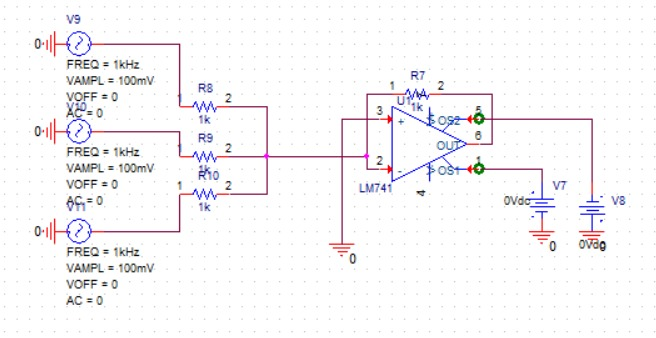
\includegraphics[scale=.5]{su.jpg}\\ 
\paragraph{Sumador}
En la imagen anterior se muestra el diagrama del circuito sumador el cual suma 3 tensiones que resulta en una sola.
\\
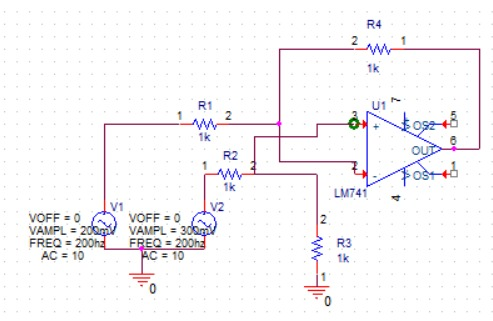
\includegraphics[scale=.5]{re.jpg} 
\paragraph{Restador}
El restador como se muestra en la imagen anterior reduce 3 tensiones en una sola que resulta ser menor a las tres primeras.
\\
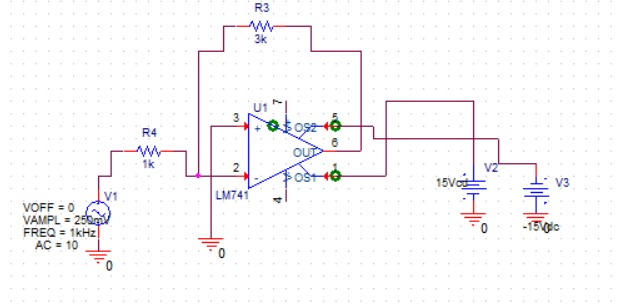
\includegraphics[scale=.5]{in.jpg} 
\paragraph{Inversor}
El circuito inversor consigue gracias al amplificador una ganacia de 2.2V calculadas por las resistencia ya que se obtine dividiendo Rf/Ri
obteniendo dicho voltaje.
\\
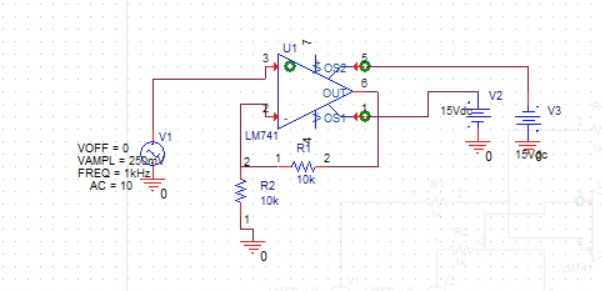
\includegraphics[scale=.5]{no in.jpg} 
\paragraph{No inversor }
Este circuito funciona similar al anterior solo que tiene la peculiaridad de aumentar mas el voltaje ya que se calcula de igual manera pero aumentando 1V mal al resultado como en esta ocacion es de 3.2V
\\
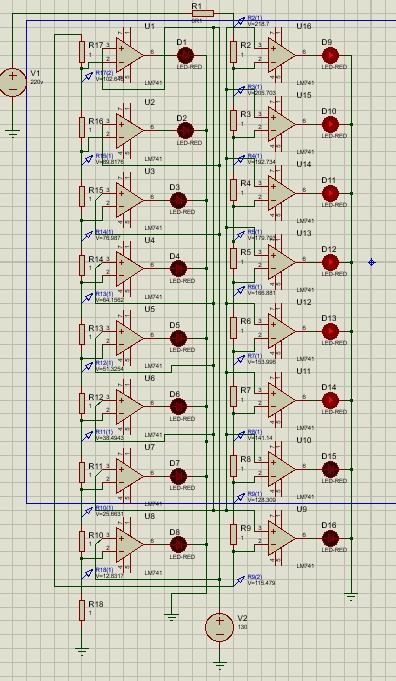
\includegraphics[scale=.5]{adc.jpg}
\paragraph{ADC}
Este circuito tiene la peculiaridad que al reducir los volts de entrada mayor cantidad de leds enciende llendo de 200V para encender un solo led hasta 10V para lograr encenderlos todos.
\\
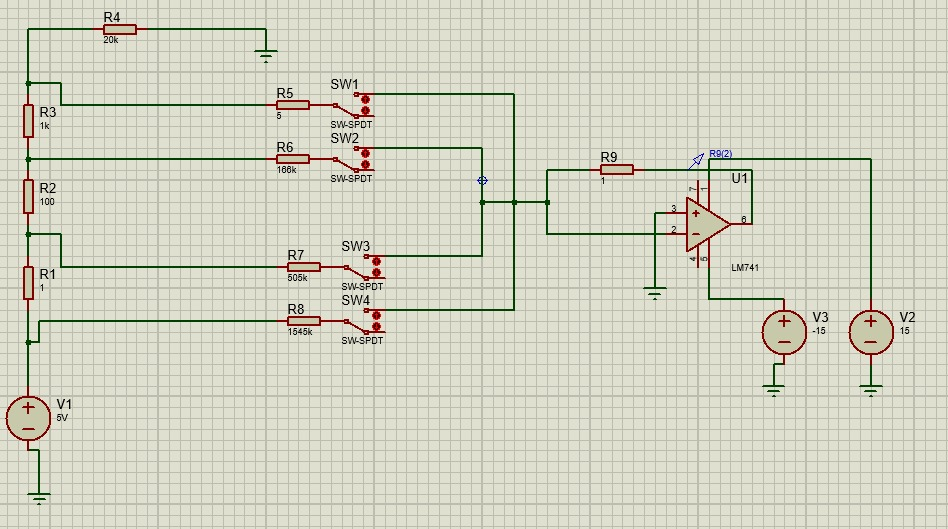
\includegraphics[scale=1]{dac.jpg}   
\paragraph{DAC}
El circuito del Dac es un circuito reductor con ase a las resistencias que lo componen ya que al tener 4 swiches cada uno reduce una cantidad de voltaje que al aver menor cantidad de ellos aplicados menor sera el voltaje de salida del amplificador.

\subsection{Conclusion }
Podemos observar como los amplifiacdores de potencia ayudan para nuestras practicas, ya que con las simulaciones podemos comprender lo que un amplificador realiza.Como su nombre lodice amplificador, este recibe una senal de alguna fuente y este amplificador manda una version amplificada de esta senal a otro dispositivo o a otra parte de este amlificador.
\\
Esta practica ayuda a comprender el funcionamiento ya visto previamente en clase de los amplificadores de potencia en los cuales nos muestra la versatilidad que estos tienen dentro de los circuirtos en los cuales tenemos que controlar las entradas y salidas de voltaje por los que los vuelven muy utiles para trabajar en proyectos en que se require dicho control para que funciones con mayor utilidad.




\end{document}